%!TEX program = xelatex
% 完整编译: xelatex -> biber/bibtex -> xelatex -> xelatex
\documentclass[lang=cn,11pt,a4paper]{elegantpaper}

\title{MLIR编译框架的使用与探索:实验报告}
\author{谢立汉 \ 519021910164 \\ sheringham@sjtu.edu.cn \and 唐亚周 \ 519021910804 \\ tangyazhou518@sjtu.edu.cn}

\institute{SJTU\ CS2301\ 编译原理(A类)}

\date{\zhtoday}

% 本文档命令
\usepackage{array}
\usepackage{float}
\newcommand{\ccr}[1]{\makecell{{\color{#1}\rule{1cm}{1cm}}}}

% 实验报告应指出实验环境(操作系统和工具版本等)
%  、实验过程、实验结果,并能完整、准确地
% 说出自己的设计思路,描述清楚各个函数的作用、具体实现方法等。总结部分可以分享自己在实验
% 过程中遇到的问题和解决方法,对 MLIR 框架的认识。也可以对大作业提出自己的意见,我们将在
% 后面的学期不断进行完善。实验报告中应写明组内两位同学的姓名、学号、联系方式及各自贡献。

\lstset{
  numbers=left,                                        % 在左侧显示行号
  numberstyle=\tiny\color{gray},                       % 设定行号格式
  language=c++,                                        % 设置语言
}


\begin{document}

\maketitle

\begin{abstract}
在本实验中,我们借助工业界先进的编译框架MLIR,完成了对基于张量的自定义语言Tiny的解析,主要包括词法分析,语法分析和代码优化三部分。在词法与语法分析部分,我们补全了Tiny语言的词法与语法分析代码,并对“var”的表示引入了新的扩展。在代码优化部分,我们对Tiny语言的\texttt{transpose()}函数进行了冗余代码消除。
\keywords{MLIR,Tiny语言,词法分析,语法分析,代码优化}
\end{abstract}


\section{引言}

\subsection{实验目的}
探索并使用当前先进的编译基础设施框架MLIR,利用课堂所学习的词法分析、语法分析以及代码优化的知识,完善基于张量的语言Tiny,重点是从编译的角度去解析这一语言。通过本次实验,熟悉MLIR框架,并且更好的将课堂所学理论知识进行巩固。
\subsection{实验环境}

虚拟机软件:Vmware

操作系统:Ubuntu 20.04

依赖工具链:\texttt{git, cmake, lld, clang, ninja}

\section{实验过程}

\subsection{基础部分}

\subsubsection{词法分析器}

在词法分析器部分,主要是实现关键字以及合法变量名的分析。其中关键字的识别包括 \texttt{return, var, def}。 而合法的变量名则需要符合如下要求 :

\begin{enumerate}
    \item 变量名以字母开头;
    \item 变量名由字母、数字、下划线组成;
    \item 变量名中有数字时,数字应位于变量名末尾,如 \texttt{a1234, b\_4, placeholder} 等。
\end{enumerate}

我们要的功能在 \texttt{getTok()} 函数中实现。首先判断当前字符是否为字母,若为字母则会进入\texttt{do while}循环,此循环不断读入下一个字符,直到非字母数字下划线为止。当出现数字时,为保证数字是变量名的结尾,将做一个标记,若接下来的字符是字母或下划线,则跳出循环,返回一个错误的token,最后当循环结束时,先判定读入的字符串是否为上述三个关键字的一种,若是则返回对应的token,不是则返回标识符的token,并且将字符串存入到 \texttt{identifierStr}中。相应代码实现如下:
\begin{lstlisting}
//TODO: Here you need to identify:
//      1. Keywords: "return", "def", "var"
//      2. Variable names
//      Note that a variable name should follow some rules:
//      1) It should start with a letter.
//      2) It consists of letters, numbers and underscores.
//      3) If there are numbers in the name, they should be at the end of the name.
//      For example, these names are valid: a123, b_4, placeholder

//Hints: 1. You can refer to the implementation of identifying a "number" in the same function.
//       2. Some functions that might be useful:  isalpha(); isalnum();
//       3. Maybe it is better for you to go through the whole lexer before you get started.

if (isalpha(lastChar)) {
    std::string varStr;
    bool no_digit = true, is_error = false;
    do {
    if (isdigit(lastChar)) {
        no_digit = false;
    }
    if (!no_digit) {
        if (isalpha(lastChar) || lastChar == '_') {
        is_error = true;
        break;
        }
    }
    varStr += lastChar;
    lastChar = Token(getNextChar());
    } while (isalnum(lastChar) || lastChar == '_');
    if (!is_error) {
    if (varStr == "return") return tok_return;
    if (varStr == "def") return tok_def;
    if (varStr == "var") return tok_var;
    identifierStr = varStr;
    return tok_identifier;
    }
}
\end{lstlisting}
\subsubsection{语法分析器}

在语法分析器的部分,该框架已经支持类似\texttt{var a}和\texttt{var a <2,3>}形式的变量定义,我们需要加上对类似\texttt{var a[2][3]}形式的变量定义的支持。我们需要修改的函数是\texttt{parseVarDeclaration}和\texttt{parseType}。

\texttt{parseVarDeclaration}函数用于对变量声明的表达式进行语法分析,其形式如下:

\begin{center}
  \texttt{var}\ \textit{identifier}\ \textbf{type}\ \texttt{=}\ \textit{expression}
\end{center}

其中的\textbf{type}指定了该矩阵的维数,可以省略这一项。

首先我们需要检查当前所在的Token是否为\texttt{tok\_var},如果不是则报错,否则就获取下一个Token(相当于“吃掉”了现在所在的Token)。接着检查当前所在的Token是否为\texttt{tok\_identifier},如果不是则报错,否则就调用在词法分析器中写的\texttt{getId}函数对其进行处理,然后处理下一个Token。然后要检查该表达式中是否有\textbf{type}这一项,将原框架中对当前Token是否为\texttt{<}的判断改成是否为\texttt{<}或\texttt{[}即可。相应的代码如下。

\begin{lstlisting}
// Parse a variable declaration,
// 1. it starts with a `var` keyword, followed by a variable name and initialization
// 2. Two methods of initialization have been supported:
//    (1) var a = [[1, 2, 3], [4, 5, 6]];
//    (2) var a <2,3> = [1, 2, 3, 4, 5, 6];
// You need to support the third method:
//    (3) var a [2][3] = [1, 2, 3, 4, 5, 6];
// Some functions may be useful:  getLastLocation(); getNextToken();
std::unique_ptr<VarDeclExprAST>
parseVarDeclaration(bool requiresInitializer) {

  auto loc = lexer.getLastLocation();

  // TODO: check to see if this is a 'var' declaration
  //       If not, report the error with 'parseError', otherwise eat 'var'

  if (lexer.getCurToken() != tok_var)
    return parseError<VarDeclExprAST>("var", "in variable declaration");
  lexer.getNextToken(); // eat var

  // TODO: check to see if this is a variable name
  //       If not, report the error with 'parseError'

  if (lexer.getCurToken() != tok_identifier)
      return parseError<VarDeclExprAST>("identified", "after 'var' declaration");

  // eat the variable name
  std::string id(lexer.getId());
  lexer.getNextToken(); // eat id

  std::unique_ptr<VarType> type;
  // TODO: modify code to additionally support the third method: var a[][] = ...
  if (lexer.getCurToken() == '<' || lexer.getCurToken() == '[') {
    type = parseType();
    if (!type)
      return nullptr;
  }
  if (!type)
    type = std::make_unique<VarType>();

  std::unique_ptr<ExprAST> expr;
  if (requiresInitializer) {
    lexer.consume(Token('='));
    expr = parseExpression();
  }
  return std::make_unique<VarDeclExprAST>(std::move(loc), std::move(id),
                                          std::move(*type), std::move(expr));
}
\end{lstlisting}

\texttt{parseType}函数用于对变量的类型(矩阵维数)进行语法分析。已有的该函数已经处理了使用\texttt{<>}符号进行声明的方式,我们需要加上对\texttt{[]}符号的支持。首先在最开始的判断中将对当前Token不为\texttt{<}的判断改成不为\texttt{<}且不为\texttt{[}。然后在对于\texttt{[]}符号的处理中,循环地处理\texttt{[}、\texttt{tok\_number}(可以为空)、\texttt{]}并不断获取下一个符号,直到当前符号不再是\texttt{[}为止。相应的代码如下。

\begin{lstlisting}
/// type ::= < shape_list >
/// shape_list ::= num | num , shape_list
// TODO: make an extension to support the new type like var a[2][3] = [1, 2, 3, 4, 5, 6];
std::unique_ptr<VarType> parseType() {
  if (lexer.getCurToken() != '<' && lexer.getCurToken() != '[')
    return parseError<VarType>("< or [", "to begin type");
  else if (lexer.getCurToken() == '<') {
    lexer.getNextToken(); // eat <

    auto type = std::make_unique<VarType>();

    while (lexer.getCurToken() == tok_number) {
      type->shape.push_back(lexer.getValue());
      lexer.getNextToken();
      if (lexer.getCurToken() == ',')
        lexer.getNextToken();
    }

    if (lexer.getCurToken() != '>')
      return parseError<VarType>(">", "to end type");
    lexer.getNextToken(); // eat >
    return type;
  } else {
    // our work for processing [] symbol
    auto type = std::make_unique<VarType>();
    while (lexer.getCurToken() == '[') {
      lexer.getNextToken(); // eat [
      if (lexer.getCurToken() == tok_number) {
        type->shape.push_back(lexer.getValue());
        lexer.getNextToken();
      }
      if (lexer.getCurToken() != ']')
        return parseError<VarType>("]", "to end shape");
      lexer.getNextToken(); // eat ]
    }
    return type;
  }
}
\end{lstlisting}


\subsection{进阶部分:代码优化}

在这一部分中,我们需要将两次矩阵转置的操作(\textit{transpose(transpose(x))})优化为没有操作(\textit{x}),从而提高代码的运行效率。根据老师给的提示可以很顺利地完成该任务。首先获得外层\textit{transpose}操作的输入\texttt{input}。然后获得它的矩阵定义操作,并判断这个定义操作是否为空。

\begin{itemize}
  \item 如果\texttt{input}是\textit{transpose(...)},那么就代表此处出现了两个连续的矩阵转置操作,可以进行优化;
  \item 如果不是,那么得到的\texttt{inputOp}就将为空,则返回\texttt{failure}并退出。
\end{itemize}

最后使用\texttt{PatternRewriter}的\texttt{replaceOp}方法,将所有出现了\texttt{op}(也就是\textit{transpose(transpose(x))})的地方都转换为\texttt{inputOp}的输入(也就是\textit{x}),这样就完成了代码优化。相应的代码如下。

\begin{lstlisting}
/// This is an example of a c++ rewrite pattern for the TransposeOp. It
/// optimizes the following scenario: transpose(transpose(x)) -> x
struct SimplifyRedundantTranspose : public mlir::OpRewritePattern<TransposeOp> {

  SimplifyRedundantTranspose(mlir::MLIRContext *context)
      : OpRewritePattern<TransposeOp>(context, /*benefit=*/1) {}

  /// TODO Redundant code elimination
  mlir::LogicalResult
  matchAndRewrite(TransposeOp op,
                  mlir::PatternRewriter &rewriter) const override {


    // Step 1: Get the input of the current transpose.
    // Hint: For op, there is a function: op.getOperand(), it returns the parameter of a TransposeOp and its type is mlir::Value.

    Value input = op.getOperand();

    // Step 2: Check whether the input is defined by another transpose. If not defined, return failure().
    // Hint: For mlir::Value type, there is a function you may use:
    //       template<typename OpTy> OpTy getDefiningOp () const
 	  //       If this value is the result of an operation of type OpTy, return the operation that defines it

    auto inputOp = input.getDefiningOp<TransposeOp>();
    if (!inputOp) return failure();

    // step 3: Otherwise, we have a redundant transpose. Use the rewriter to remove redundancy.
    // Hint: For mlir::PatternRewriter, there is a function you may use to remove redundancy:
    //       void replaceOp (mlir::Operation *op, mlir::ValueRange newValues)
    //       Operations of the second argument will be replaced by the first argument.

    rewriter.replaceOp(op, {inputOp.getOperand()});

    return success();
  }
};
\end{lstlisting}

\section{实验结果}

\begin{enumerate}
  \item 基础部分:词法分析器

  结果如图\ref{fig1}所示。可以看到,对于这四个有语法错误的测试用例,我们能够正确地输出错误的词法单元。
  \begin{figure}[H]
    \centering
    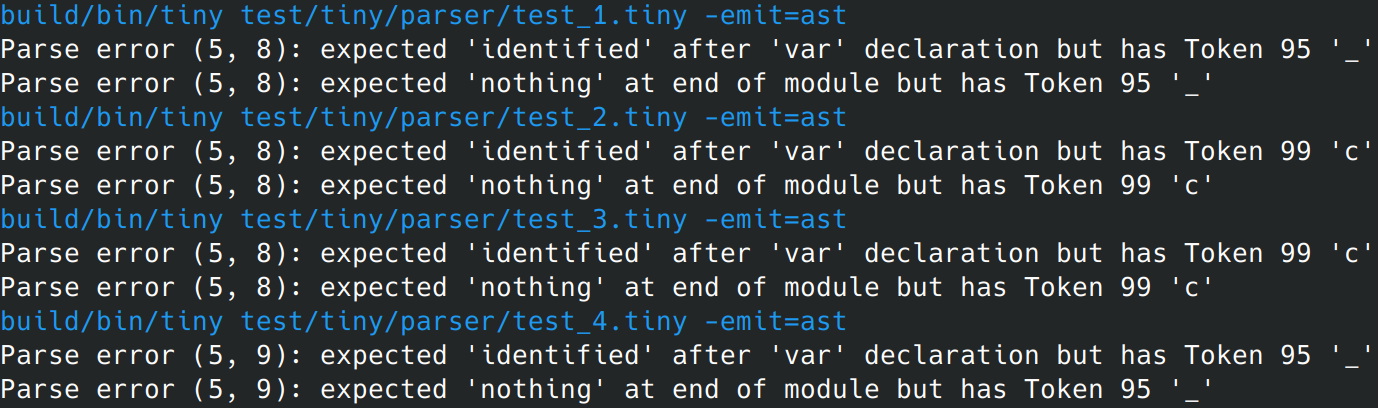
\includegraphics[width=0.9\textwidth]{./img/test1-4.png}
    \caption{Test 1 \textasciitilde Test 4的测试结果}
    \label{fig1}
  \end{figure}

  \item 基础部分:语法分析器

  结果如图\ref{fig2}所示。可以看到,对于这两个测试用例,我们能够正确地输出语法分析得到的AST,也可以输出程序的运行结果。

  \begin{figure}[H]
    \centering
    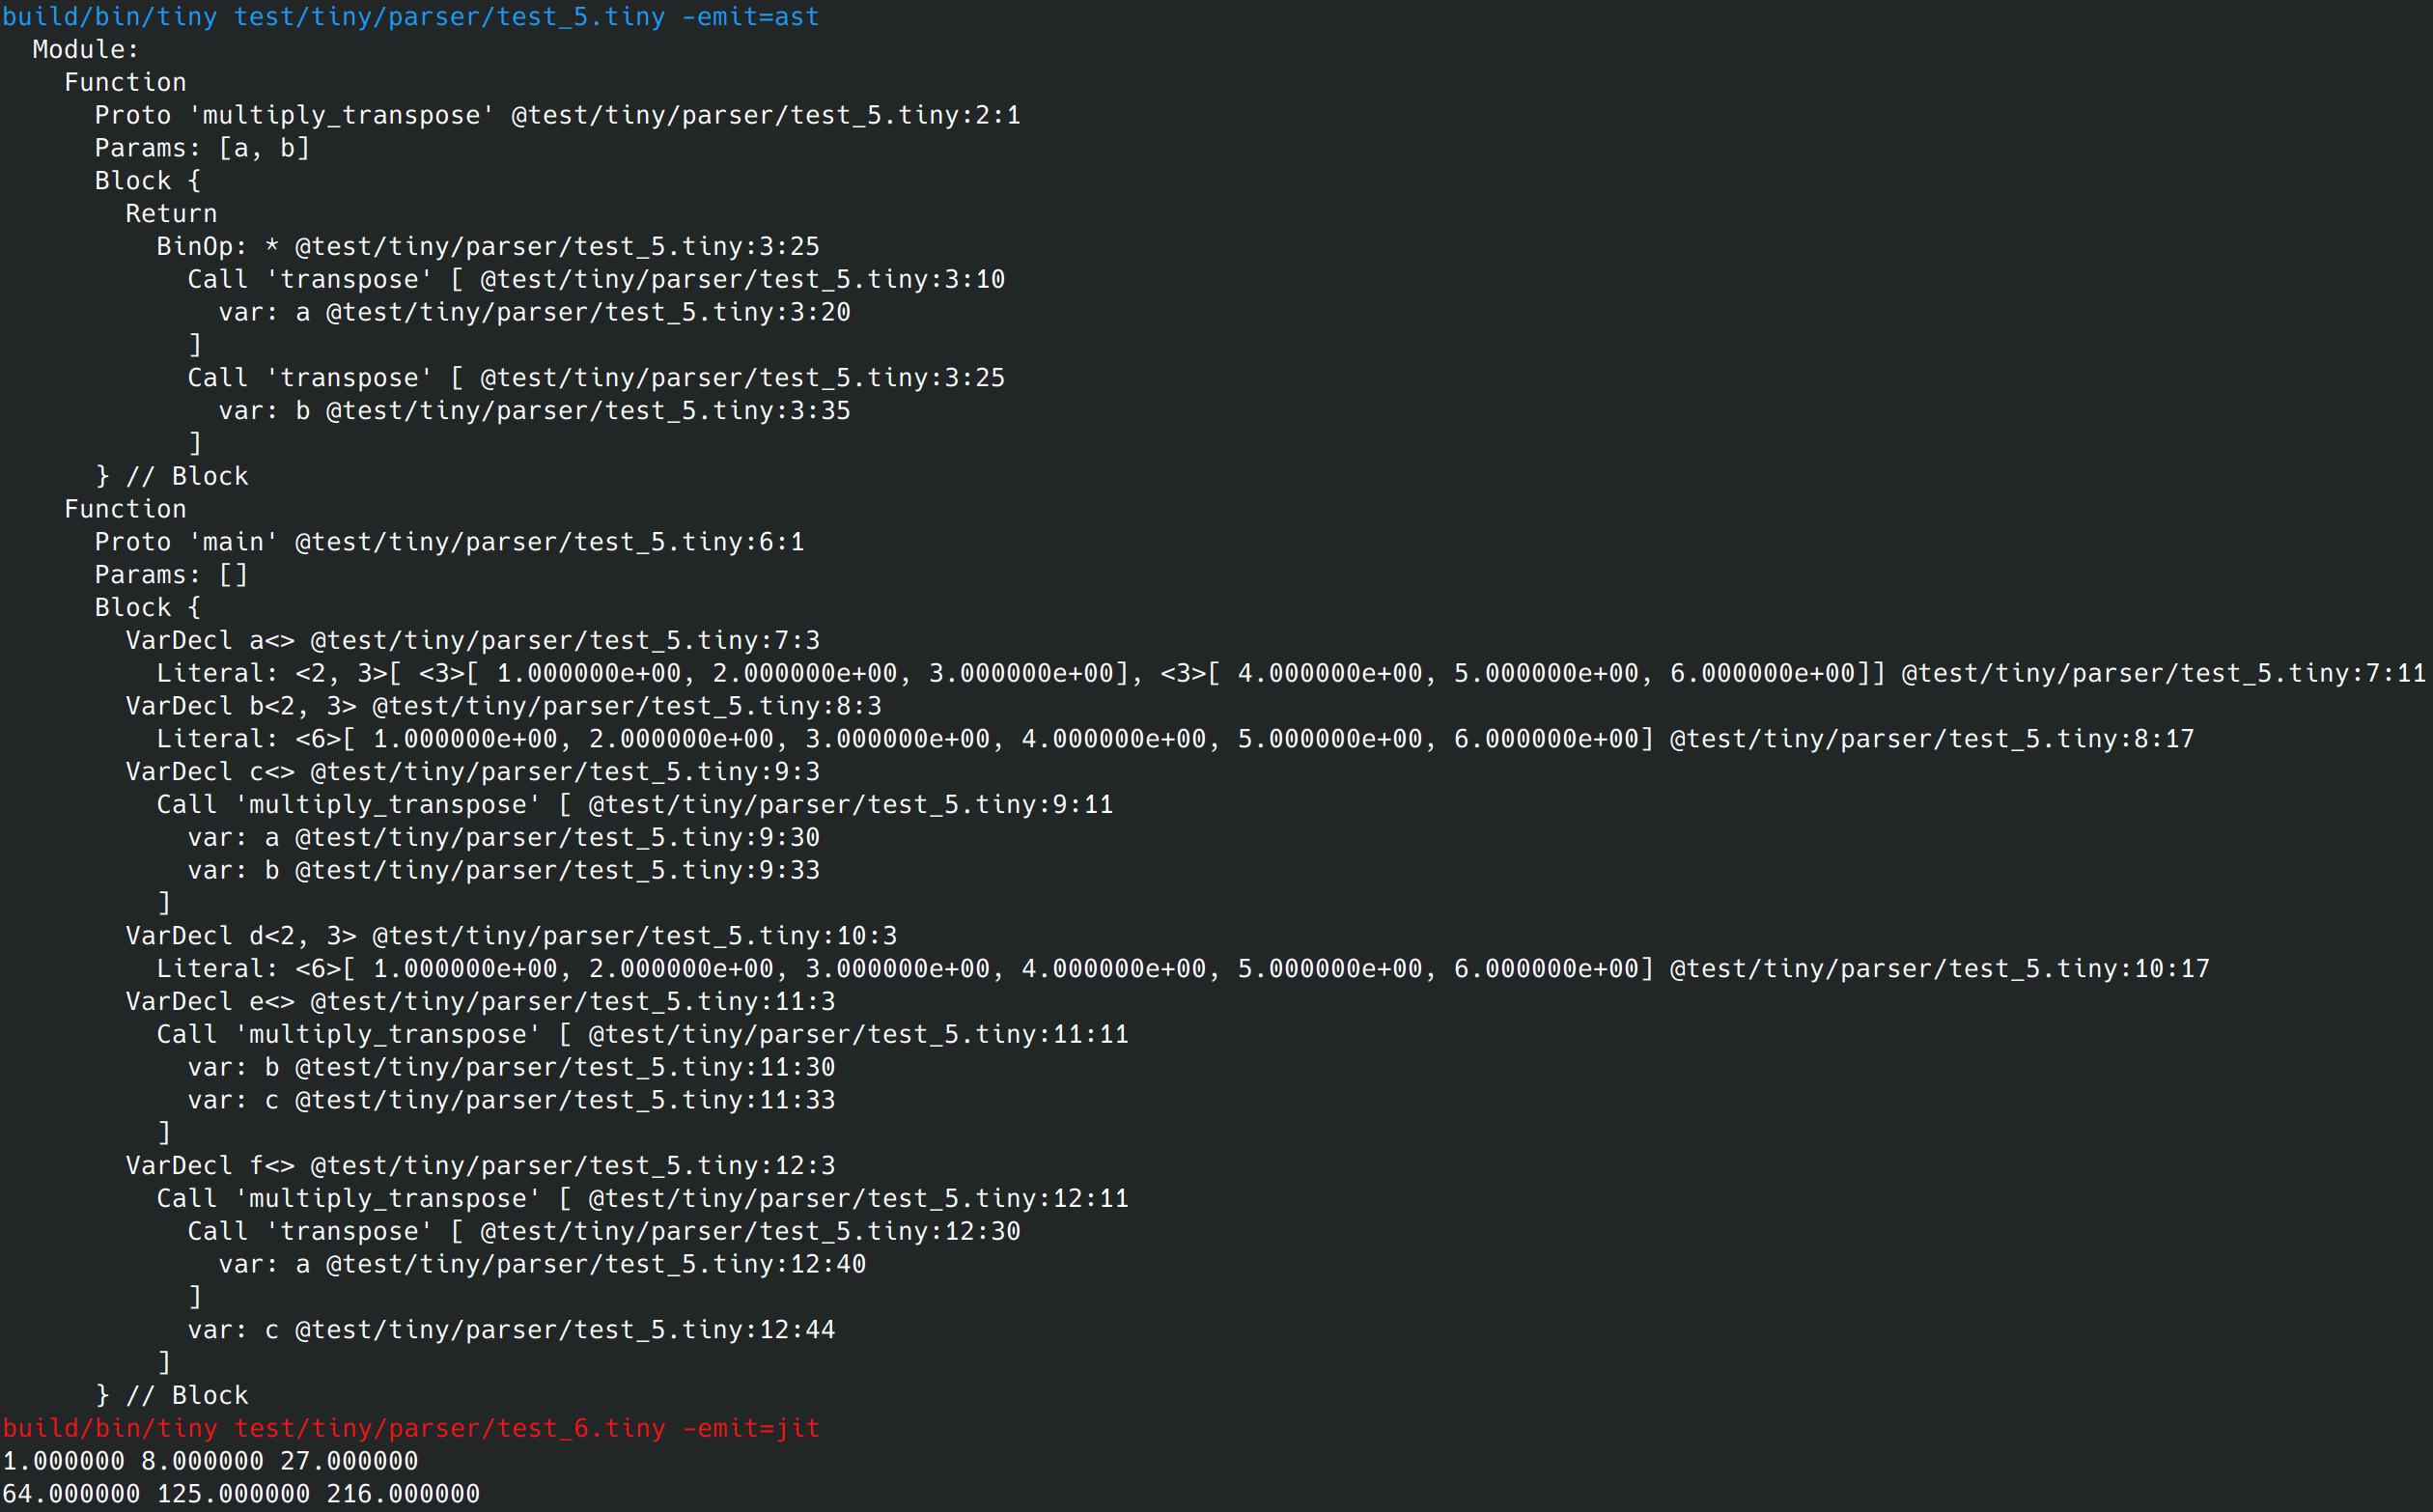
\includegraphics[width=0.9\textwidth]{./img/test5-6.png}
    \caption{Test 5和Test 6的测试结果}
    \label{fig2}
  \end{figure}

  \item 进阶部分:代码优化

  优化前后的结果分别如图\ref{fig3}和图\ref{fig4}所示。可以看到,对于这个测试用例,优化前后的AST和执行结果都是一样的,但生成的MLIR代码不同。优化后的程序与优化前相比,它输出的MLIR代码少了两次冗余的矩阵转置运算,说明我们的实现是正确的。

  \begin{figure}[H]
    \centering
    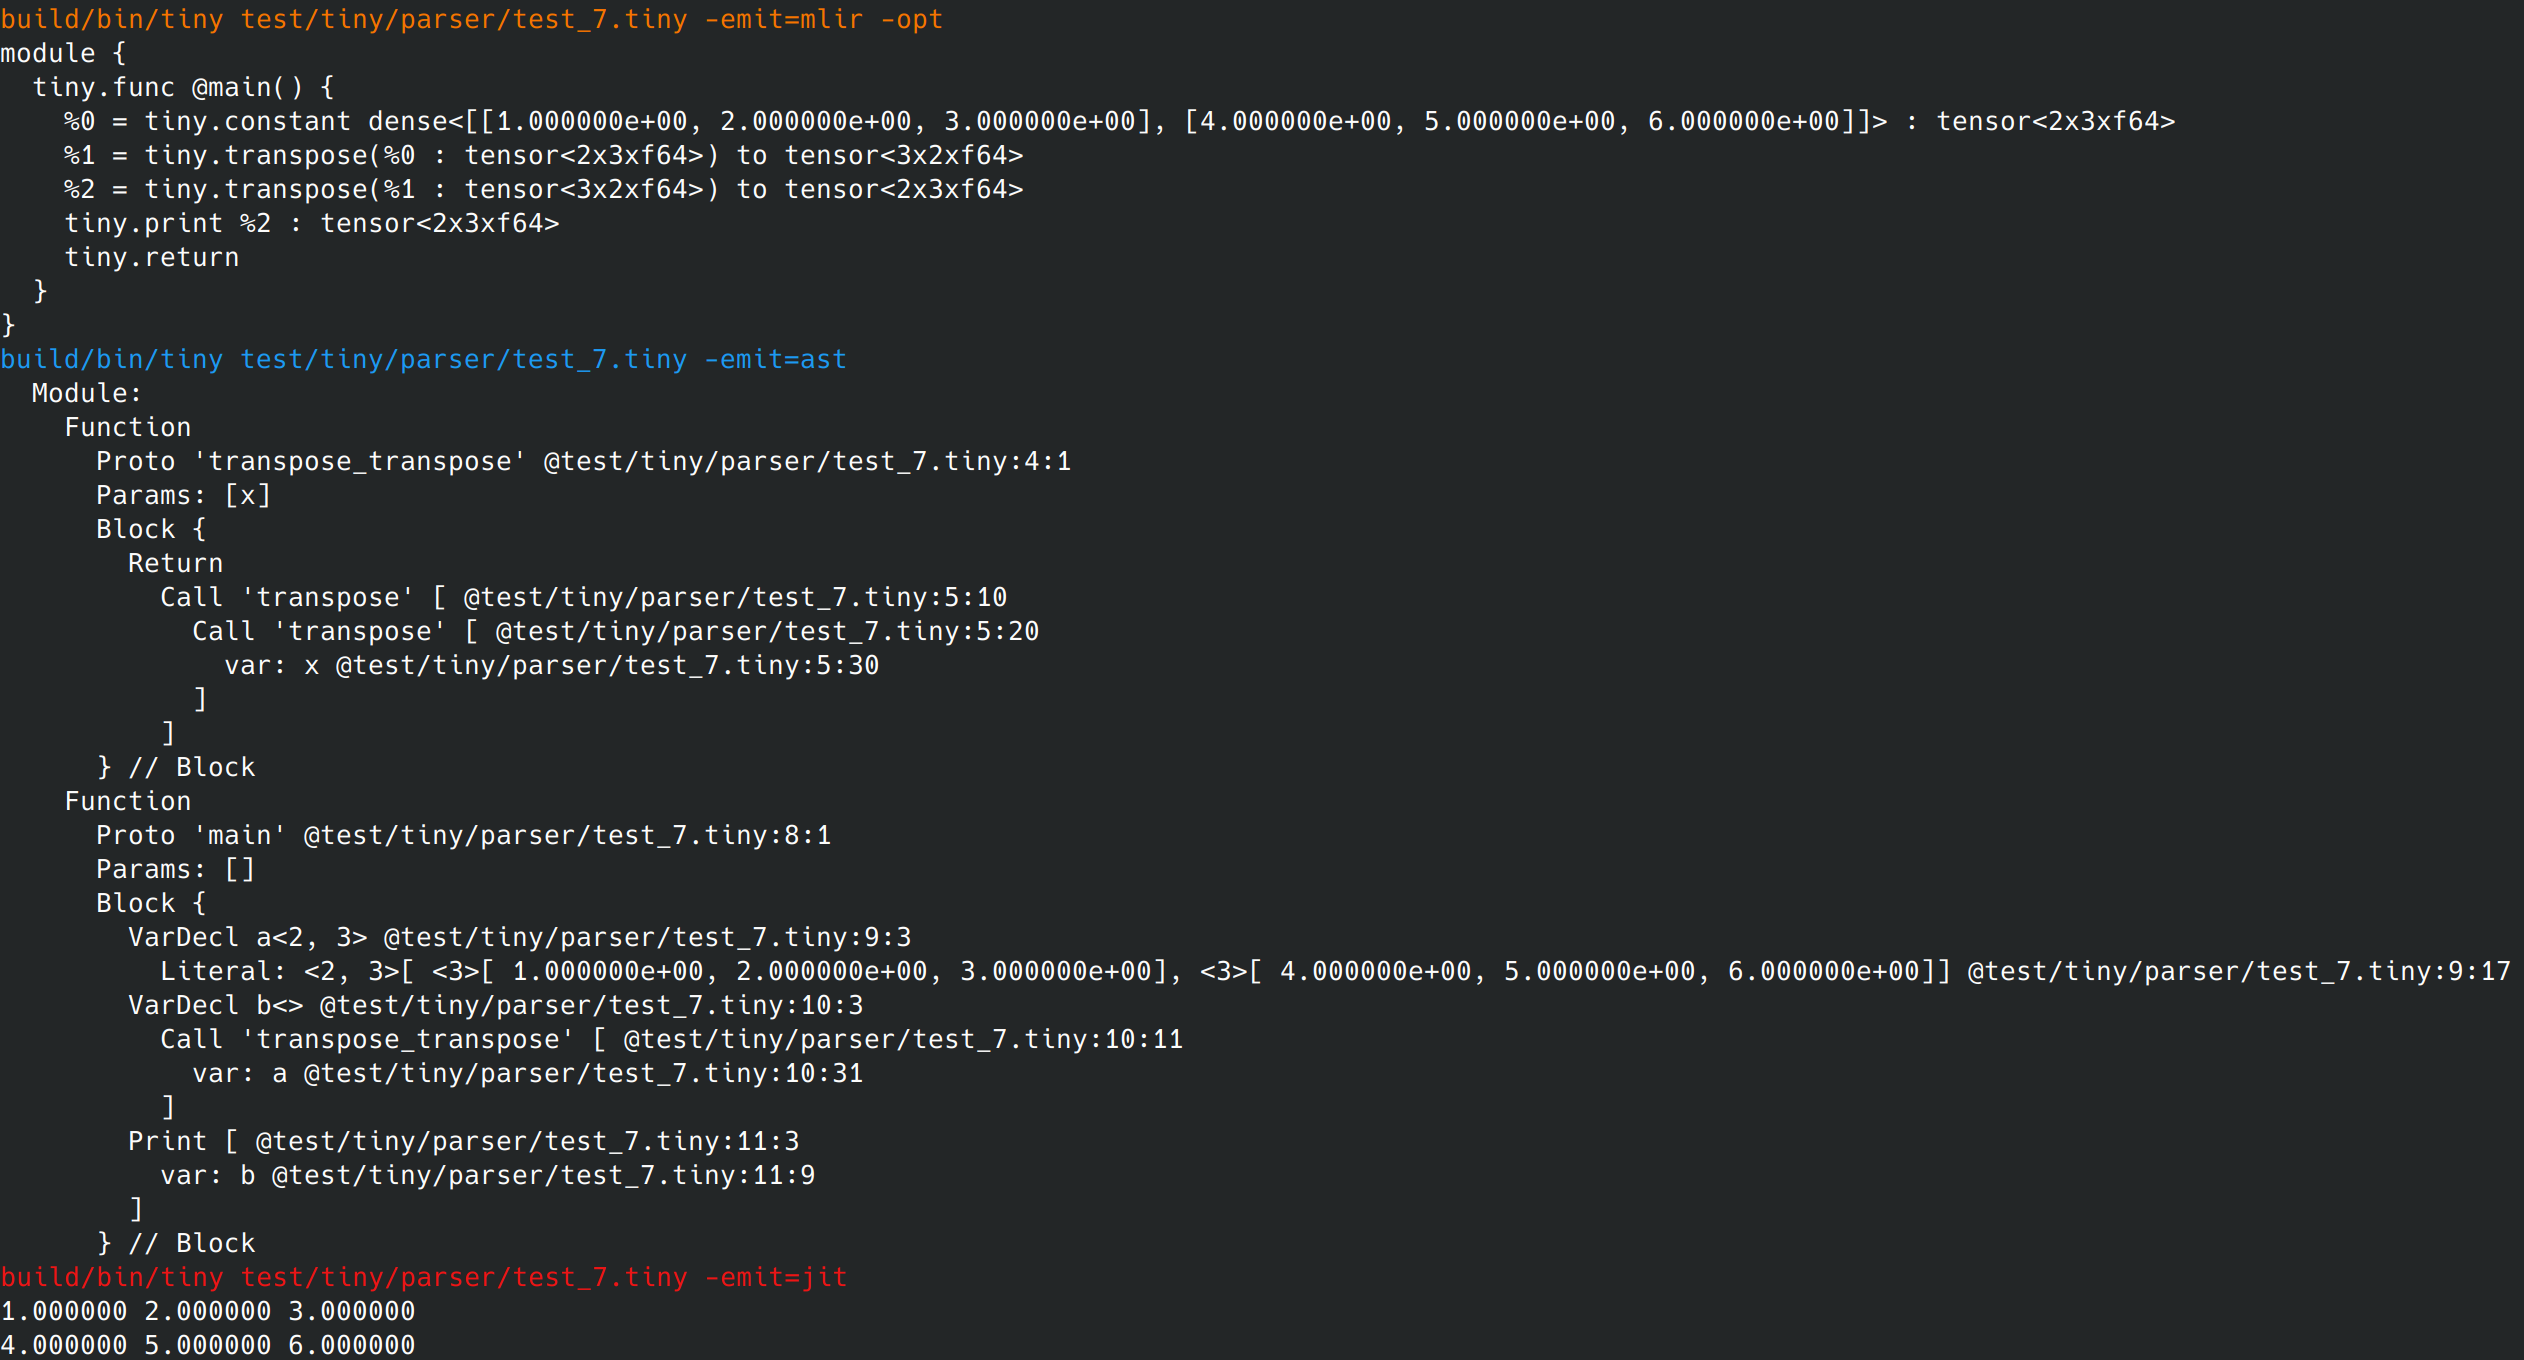
\includegraphics[width=0.9\textwidth]{./img/test7-unoptimized.png}
    \caption{Test 7的测试结果(优化矩阵转置前)}
    \label{fig3}
  \end{figure}

  \begin{figure}[H]
    \centering
    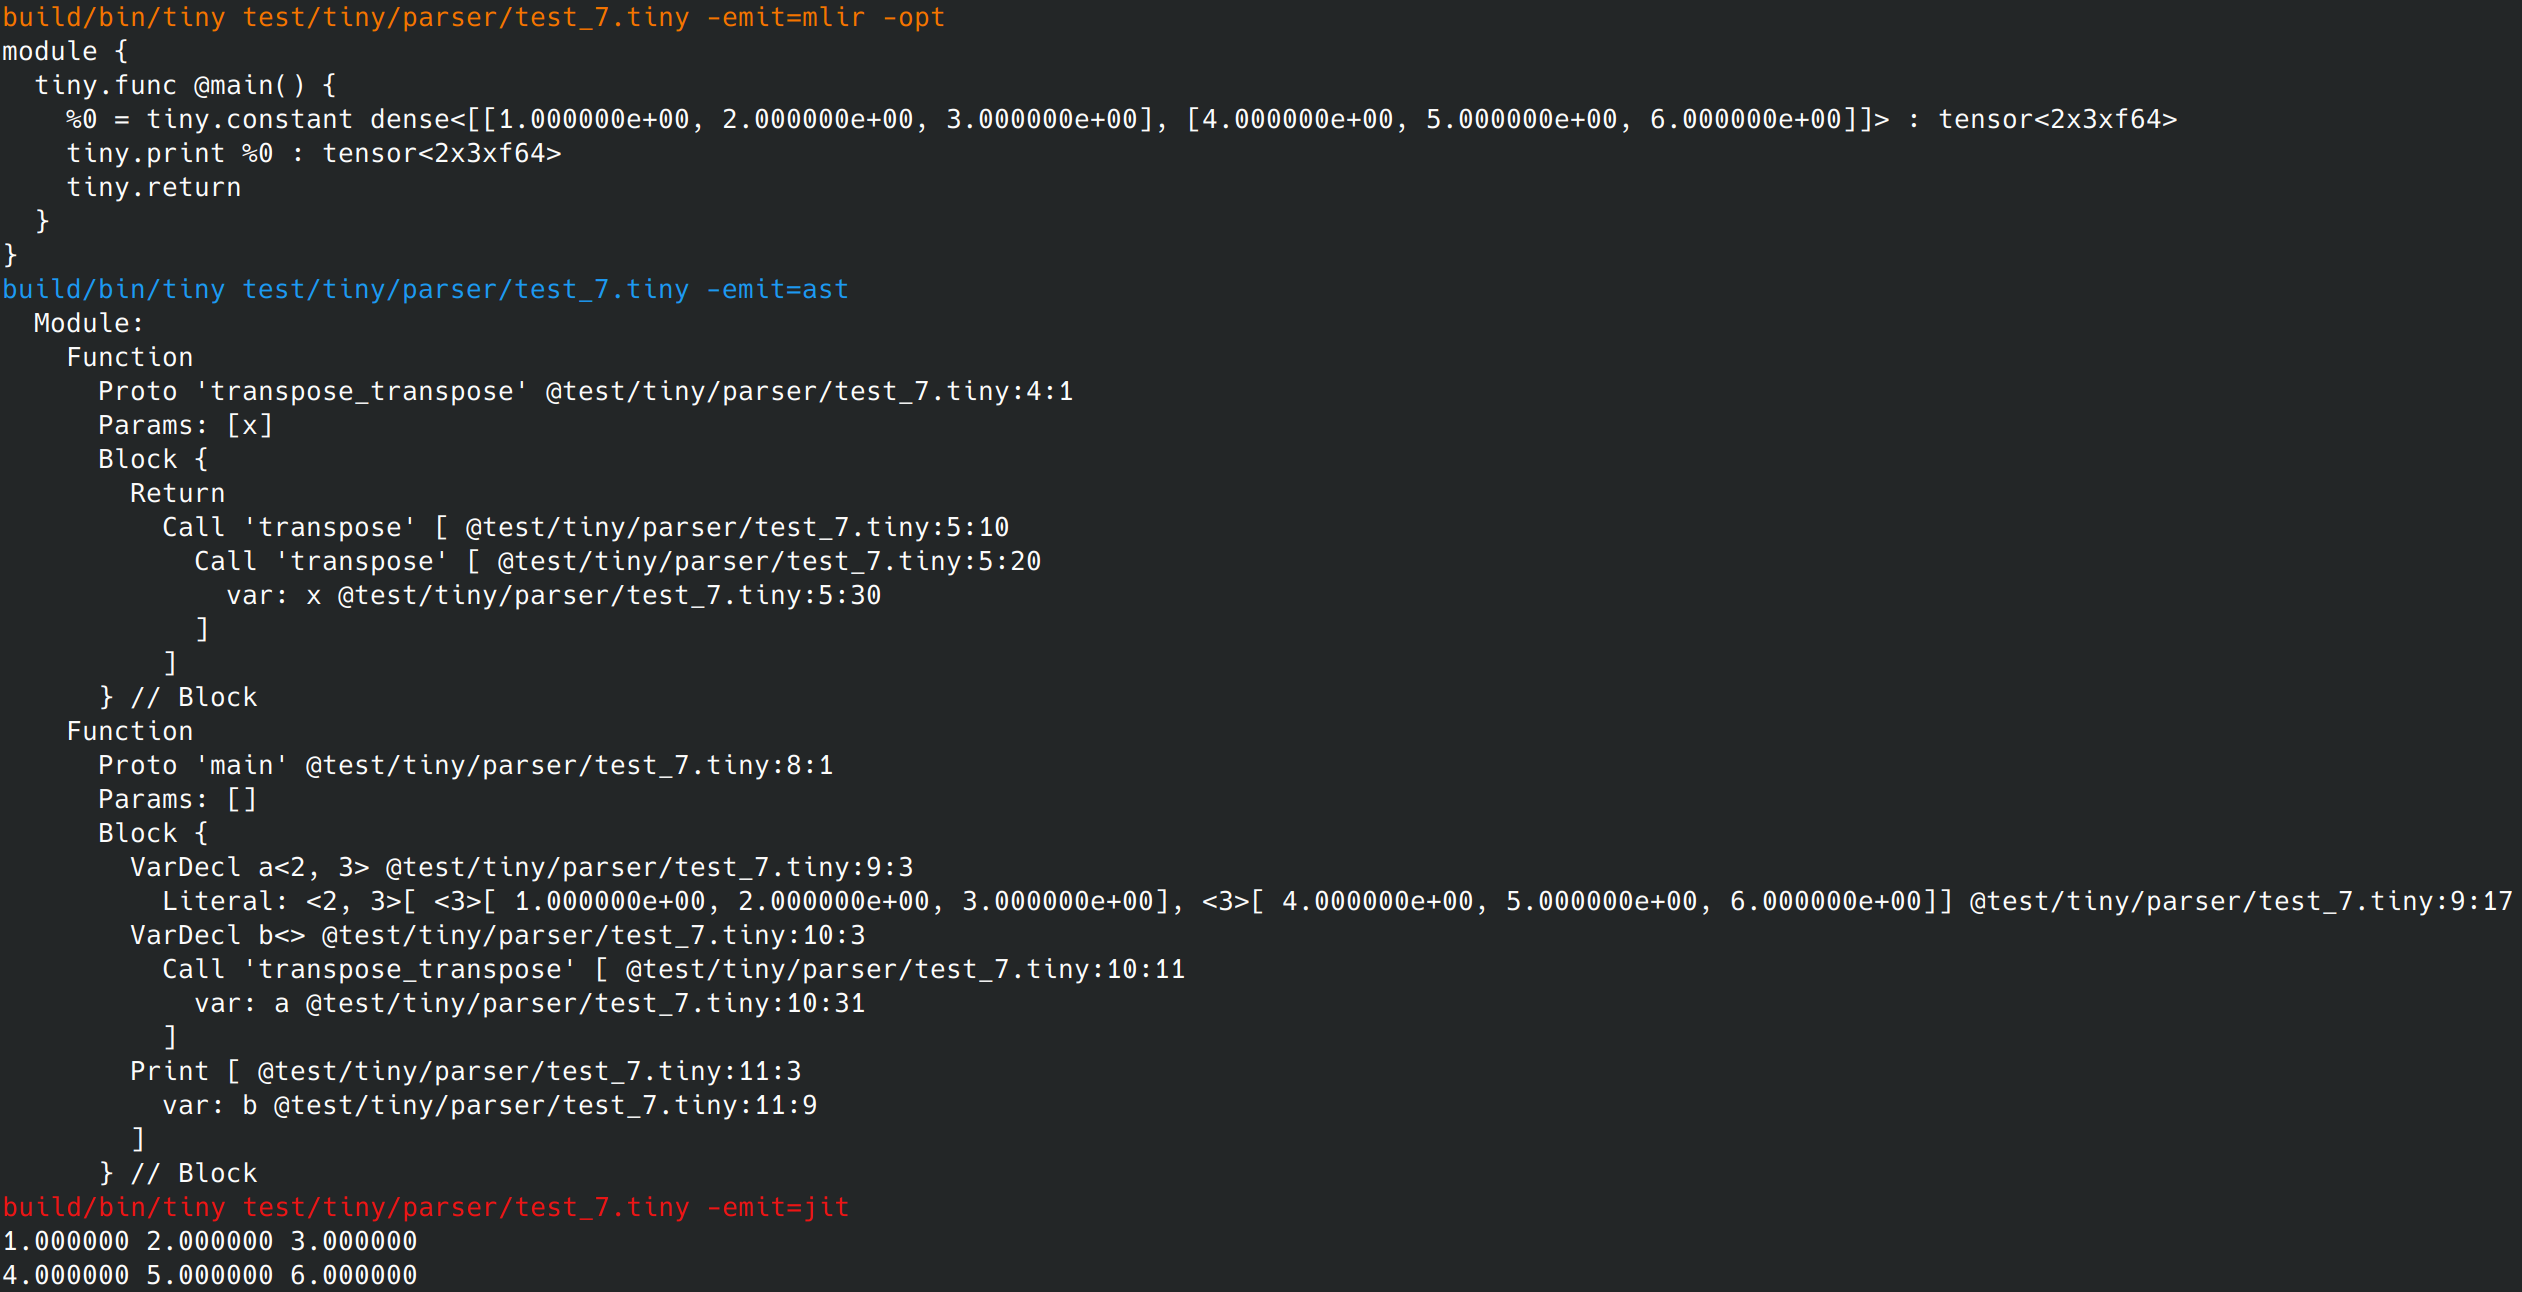
\includegraphics[width=0.9\textwidth]{./img/test7-optimized.png}
    \caption{Test 7的测试结果(优化矩阵转置后)}
    \label{fig4}
  \end{figure}

\end{enumerate}



\section{总结}

% 自己在实验过程中遇到的问题和解决方法,对 MLIR 框架的认识。也可以对大作业提出自己的意见

总的来说,我们感觉本次实验的难度并不大(可能因为我们是大三的学生),但我们中途也遇到并成功解决了以下两个问题。

首先是微信群里有好几位同学讨论过的,关于词法分析器报错Assertion failed的问题。我们一开始对整个框架的错误处理感到困惑,但在仔细阅读整体源码后,发现词法分析器中的\texttt{getTok}函数会将所有不能识别的词法单元直接以其ASCII码的形式返回,然后我们就可以在语法分析器中发现这个错误,并在语法分析器中打印错误信息,从而可以准确地指出错误的词法单元,满足了实验要求。

其次是关于代码优化部分的第三步,我们根据官方文档完成了代码之后,却感觉好像注释中的提示有些矛盾。在和同学讨论了之后,我们觉得有可能是注释写错了,在与助教交流后才发现确实是提示写错了。

对于这个大作业,我们感觉还是偏简单了一些。如果能够根据课程进度来分阶段布置大作业,然后将TODO的范围扩大,可能会更好一些。以下是我们的一些想法。
\begin{itemize}
    \item 比如在讲语法分析的时候布置语法分析器部分、讲词法分析的时候布置词法分析器部分,并且只给出各个函数的实现要求(功能、输入形式、输出形式等)来让大家实现这些函数,而不是只在某个函数中挖一个TODO。这样的话,大家在平时学习理论的过程中也能进行实践,对知识的印象也会更深一些,这可能比仅仅做龙书的课后习题要好一些。而且给出了框架,再搭配上一些tutorial,就不至于让大家从零开始,也保证了其友好性。
    \item 由于我们这个课程的重点还是在前端,所以对于中间代码生成和后端的代码优化,就可以类似于目前的形式,挖几个TODO让大家做。
\end{itemize}

对于MLIR框架,我们通过官方文档和知乎、博客等,大概有了一些了解,但也仅限于作业用到的部分了。之后有时间会继续深入学习的。

\section{致谢}

感谢赵杰茹和蒋力两位老师一个学期以来的指导,感谢张炜创和黄世远两位助教学长一学期以来的帮助。在这门课上,我们学到了许多编译器相关的知识,并对这方面产生了浓厚的兴趣。

\renewcommand\refname{参考文献}
\begin{thebibliography}{99}

\bibitem{ref1} Code Documentation - MLIR \href{https://mlir.llvm.org/docs/}{https://mlir.llvm.org/docs/}

\bibitem{ref2} MLIR 文章视频汇总 - 知乎 \href{https://zhuanlan.zhihu.com/p/141256429}{https://zhuanlan.zhihu.com/p/141256429}

\end{thebibliography}


\appendix
\appendixpage
\addappheadtotoc

组内分工:其实我们比较快地就完成了这个实验,所以也没有很明确地分工。大致情况如下。

\begin{itemize}
  \item 谢立汉:词法分析部分的代码+报告,以及报告的引言部分。
  \item 唐亚周:语法分析和代码优化部分而的代码+报告,以及报告的测试和总结部分。
\end{itemize}

\end{document}
